\usetikzlibrary{decorations.pathreplacing}
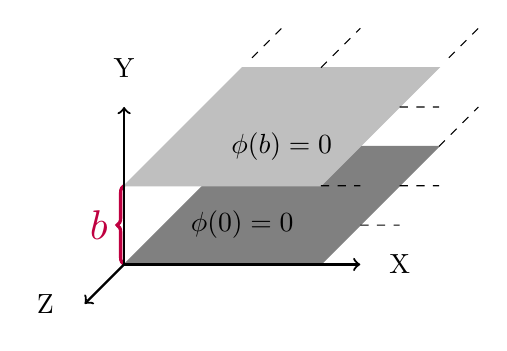
\begin{tikzpicture}
\draw [fill, gray](1,-1) -- (3.5,-1) -- (5,0.5) -- (2.5,0.5) -- (1,-1);
\draw [fill, lightgray](1,0) -- (3.5,0) -- (5,1.5) node (v2) {} -- (2.5,1.5) node (v1) {} -- (1,0);
\draw [decorate, decoration=brace, draw=purple, very thick](1,-1)--(1,0)  node [midway, left, purple, scale=1.5]{$b$};
\draw [thick, <->](1,1) -- (1,-1) -- (4,-1);
\draw [thick, ->](1,-1) -- (0.5,-1.5);
\node at (4.5,-1) {X};
\node at (1,1.5) {Y};
\node at (0,-1.5) {Z};
\draw [dashed](v1) -- (3,2);
\draw [dashed] (3.5,1.5) -- (4,2) (v2) -- (5.5,2) (5,0.5) -- (5.5,1) (4,-0.5) -- (4.5,-0.5) (4.5,0) -- (5,0) (4.5,1) -- (5,1) (3.5,0) -- (4,0);
\node at (3,0.5) {$\phi(b) =0$};
\node at (2.5,-0.5) {$\phi(0) =0$};
\end{tikzpicture}